\chapter{Track Reconstruction}
\label{sec:track}
	The~first stage of our reconstruction algorithm is the~reconstruction of the track of the~primary particle (electron or positron). The~results of this step are then used to determine the~energy of the~particle (see section~\ref{sec:energy}).
	
	\textbf{First Attempts} at a~track reconstruction were made using the~standard approach. Here we assume we know the~readout coordinates ($x'$,~$y'$,~$t$) exactly (i.e. we neglect the~pads and time bins). In standard TPC (with parallel fields) we only need to reconstruct the~$z$~coordinate from drift time using the~known drift velocity.
	
	Reconstruction with the~\textbf{Ionization Electron Map} (from now on referred to as \emph{the~map}) uses simulation of the~drift of the~secondary (ionization) electrons in the~volume of the detector. This simulation can then be used to interpolate the~initial position of the~secondary electrons. First attempts neglect the~pads.
	
	The~\textbf{Discrete Reconstruction} is made using the~map, instead of reconstructing the~exact position of each electron we reconstruct the middle point of each hit pad with time corresponding to the~middle of the~time bin. The number of electrons in each TPC~bin (consisting of the~pad and the~time bin) is counted and used as a~charge in the~energy reconstruction.
	
	\textcolor{red}{Reconstruction of one track simulated with microscopic tracking in Garfield++.}
	
	\section{First Attempts}
		\textcolor{red}{Using the same method as in standard TPC (calculating $z$ from the drift time). Gas composition 90/10.}
		
		\begin{figure}
			\centering
			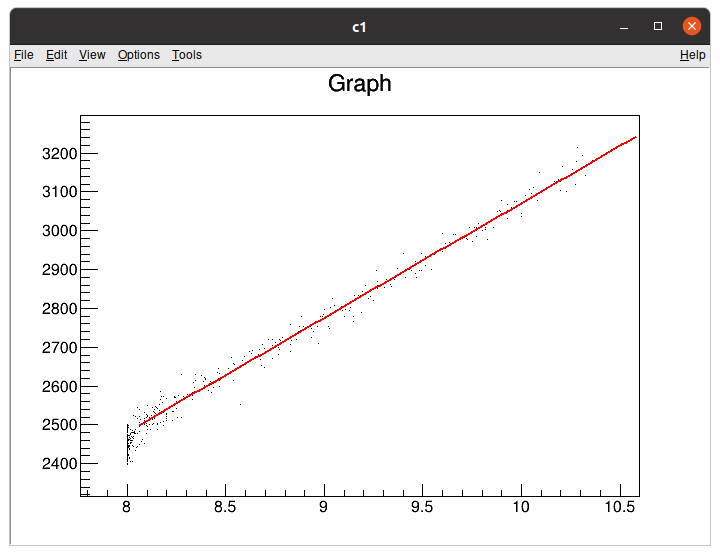
\includegraphics[width=0.5\textwidth]{9010_zt.png}
			\caption{Dependence of the~drift time on the~$z$~coordinate in 90~\%~argon and 10~\%~CO$_2$ atmosphere, fitted with a~linear function. The~fitted function gives us the~average drift velocity in the~gas and can be used for rough reconstruction in our TPC. \textcolor{red}{Swap for better image with axis labels, etc. Maybe write the~fitted equation.}}
			\label{fig:9010zt}
		\end{figure}
		
		\begin{figure}
			\centering
			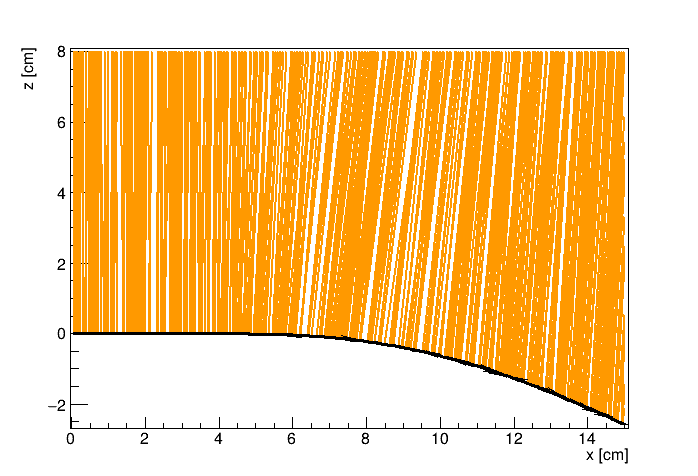
\includegraphics[width=0.5\textwidth]{9010_xz.png}
			\caption{First attempt at a~track reconstruction using only the~drift velocity. This approach works well in a~standard TPC (\textcolor{red}{ideally cite some source?}). 90~\%~argon and 10~\%~CO$_2$ atmosphere. \textcolor{red}{Swap for better image, correct coordinates.}}
			\label{fig:9010xz}
		\end{figure}
		
		\begin{figure}
			\centering
			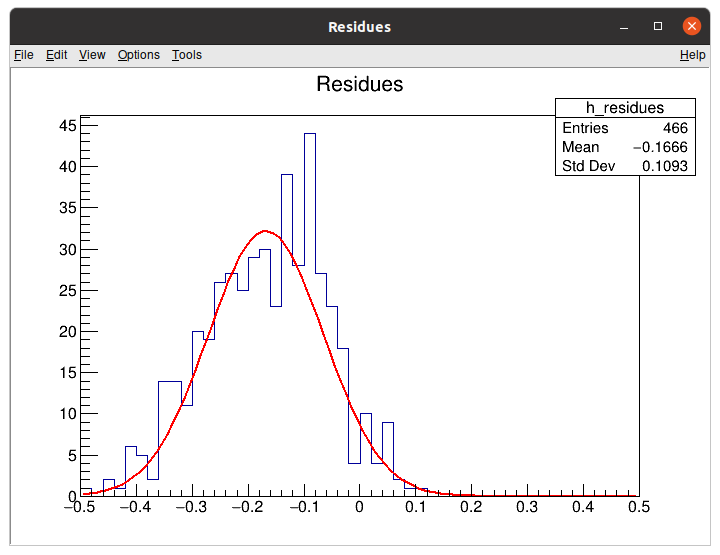
\includegraphics[width=0.5\textwidth]{9010_res.png}
			\caption{First attempt at a~track reconstruction using only the~drift velocity, residues. \textcolor{red}{Swap for better image, correct coordinates. What's causing the shift? Explain details.}}
			\label{fig:9010res}
		\end{figure}
	
	\section{Ionization Electron Map}
	\label{sec:map}
		\textcolor{red}{Explanation of the map. Simulated on MetaCentrum, workload distribution between multiple jobs. More electrons at one location to get statistics. Two methods of reconstruction using this map. Comparison of 90/10 and 70/30 maps.}
		
		\begin{figure}
			\centering
			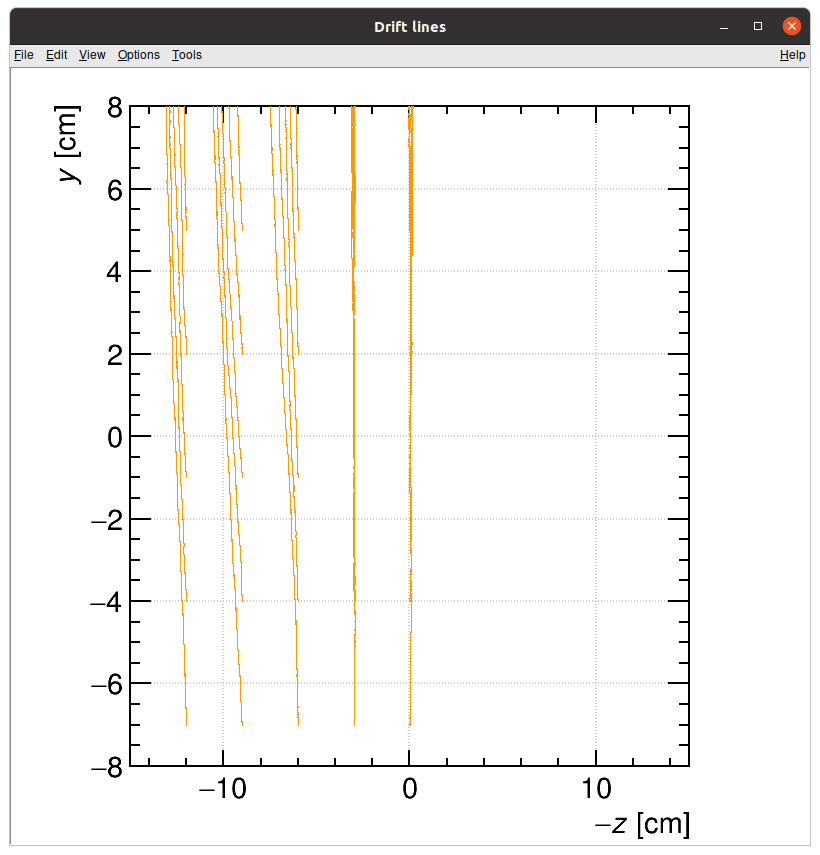
\includegraphics[width=0.5\textwidth]{map_9010_gen.png}
			\caption{Example of map generation. \textcolor{red}{Swap for better image, correct coordinates.}}
			\label{fig:map9010gen}
		\end{figure}
		
		\begin{figure}
			\centering
			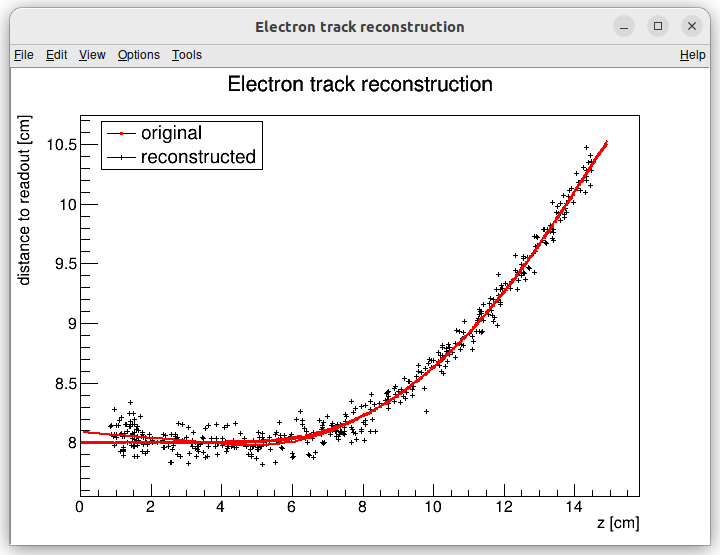
\includegraphics[width=0.5\textwidth]{9010_reco.png}
			\caption{Example reconstruction with the map. \textcolor{red}{Swap for better image, correct coordinates.}}
			\label{fig:9010reco}
		\end{figure}
		
		\subsection{Gradient Descent Search}
			\textcolor{red}{Gradient descent search of a point in the original space that gets mapped to the given point of the readout space (trilinear interpolation).}
			
			\subsubsection{Trilinear Interpolation}
			\textcolor{red}{\newline Explanation of trilinear interpolation.}
		
		\subsection{Interpolating in the Inverse Grid}
			\textcolor{red}{Interpolating between known points in the readout space. Gaussian elimination, multivariate polynomial.}
			
			\begin{figure}
				\centering
				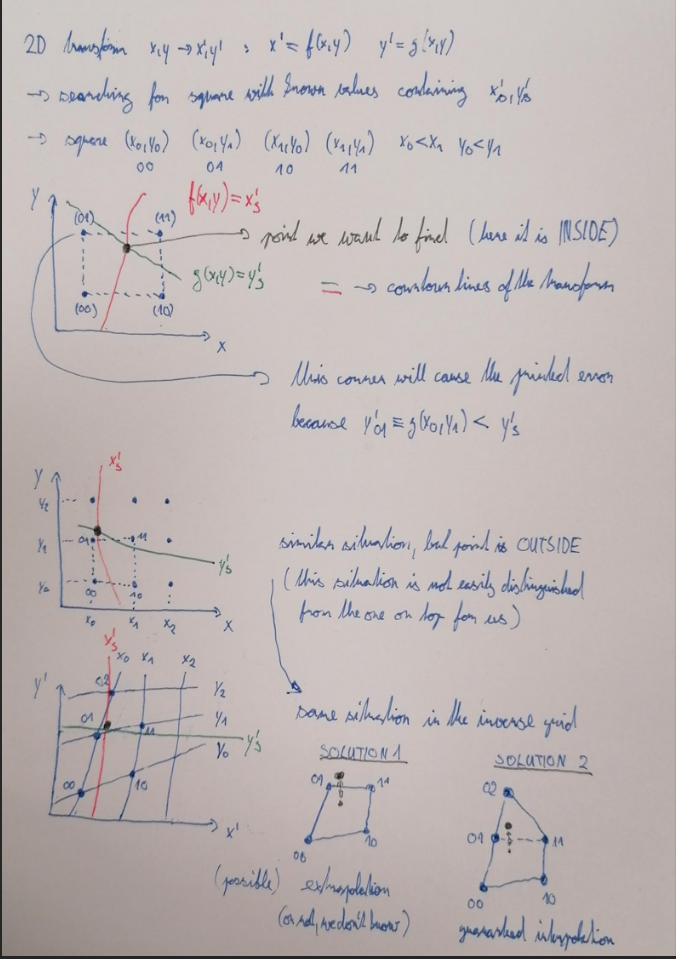
\includegraphics[width=0.8\textwidth]{interpol.png}
				\caption{Selection of the points for interpolation. \textcolor{red}{Create better images, use the explanation interpolation vs extrapolation strange property. Solution~2 probably does not make much sense.}}
				\label{fig:interpol}
			\end{figure}
		
	\section{Discrete Reconstruction}
		\textcolor{red}{Reconstruction with pads and time bins. Maybe testing different pads.}